\chapter{The Hundred Days}

M. Noirtier was a true prophet, and things progressed rapidly, as he
had predicted. Everyone knows the history of the famous return from
Elba, a return which was unprecedented in the past, and will probably
remain without a counterpart in the future.

Louis XVIII. made but a faint attempt to parry this unexpected blow;
the monarchy he had scarcely reconstructed tottered on its precarious
foundation, and at a sign from the emperor the incongruous structure of
ancient prejudices and new ideas fell to the ground. Villefort,
therefore, gained nothing save the king’s gratitude (which was rather
likely to injure him at the present time) and the cross of the Legion
of Honor, which he had the prudence not to wear, although M. de Blacas
had duly forwarded the brevet.

Napoleon would, doubtless, have deprived Villefort of his office had it
not been for Noirtier, who was all powerful at court, and thus the
Girondin of ’93 and the Senator of 1806 protected him who so lately had
been his protector. All Villefort’s influence barely enabled him to
stifle the secret Dantès had so nearly divulged. The king’s procureur
alone was deprived of his office, being suspected of royalism.

However, scarcely was the imperial power established—that is, scarcely
had the emperor re-entered the Tuileries and begun to issue orders from
the closet into which we have introduced our readers,—he found on the
table there Louis XVIII.’s half-filled snuff-box,—scarcely had this
occurred when Marseilles began, in spite of the authorities, to
rekindle the flames of civil war, always smouldering in the south, and
it required but little to excite the populace to acts of far greater
violence than the shouts and insults with which they assailed the
royalists whenever they ventured abroad.

\begin{figure}[ht]
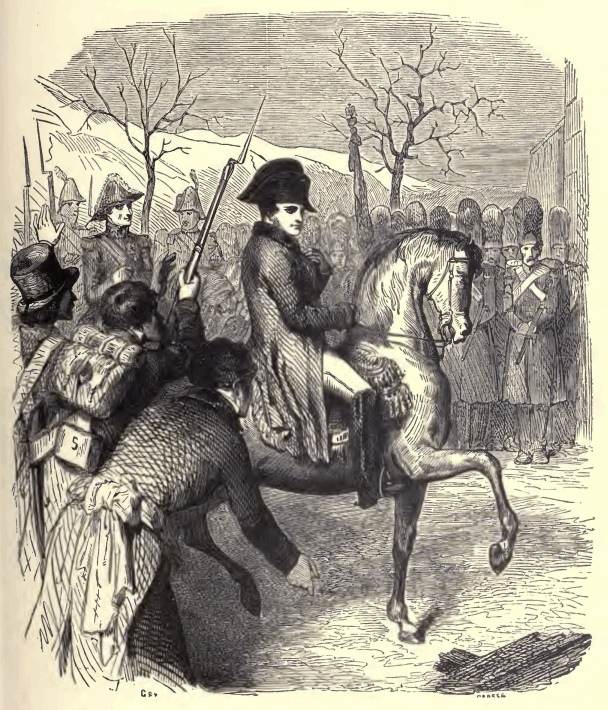
\includegraphics[width=\textwidth]{0159m.jpg}
\end{figure}

Owing to this change, the worthy shipowner became at that moment—we
will not say all powerful, because Morrel was a prudent and rather a
timid man, so much so, that many of the most zealous partisans of
Bonaparte accused him of “moderation”—but sufficiently influential to
make a demand in favor of Dantès.

Villefort retained his place, but his marriage was put off until a more
favorable opportunity. If the emperor remained on the throne, Gérard
required a different alliance to aid his career; if Louis XVIII.
returned, the influence of M. de Saint-Méran, like his own, could be
vastly increased, and the marriage be still more suitable. The deputy
procureur was, therefore, the first magistrate of Marseilles, when one
morning his door opened, and M. Morrel was announced.

Anyone else would have hastened to receive him; but Villefort was a man
of ability, and he knew this would be a sign of weakness. He made
Morrel wait in the antechamber, although he had no one with him, for
the simple reason that the king’s procureur always makes everyone wait,
and after passing a quarter of an hour in reading the papers, he
ordered M. Morrel to be admitted.

Morrel expected Villefort would be dejected; he found him as he had
found him six weeks before, calm, firm, and full of that glacial
politeness, that most insurmountable barrier which separates the
well-bred from the vulgar man.

He had entered Villefort’s office expecting that the magistrate would
tremble at the sight of him; on the contrary, he felt a cold shudder
all over him when he saw Villefort sitting there with his elbow on his
desk, and his head leaning on his hand. He stopped at the door;
Villefort gazed at him as if he had some difficulty in recognizing him;
then, after a brief interval, during which the honest shipowner turned
his hat in his hands,

“M. Morrel, I believe?” said Villefort.

“Yes, sir.”

“Come nearer,” said the magistrate, with a patronizing wave of the
hand, “and tell me to what circumstance I owe the honor of this visit.”

“Do you not guess, monsieur?” asked Morrel.

“Not in the least; but if I can serve you in any way I shall be
delighted.”

“Everything depends on you.”

“Explain yourself, pray.”

“Monsieur,” said Morrel, recovering his assurance as he proceeded, “do
you recollect that a few days before the landing of his majesty the
emperor, I came to intercede for a young man, the mate of my ship, who
was accused of being concerned in correspondence with the Island of
Elba? What was the other day a crime is today a title to favor. You
then served Louis XVIII., and you did not show any favor—it was your
duty; today you serve Napoleon, and you ought to protect him—it is
equally your duty; I come, therefore, to ask what has become of him?”

\begin{figure}[ht]
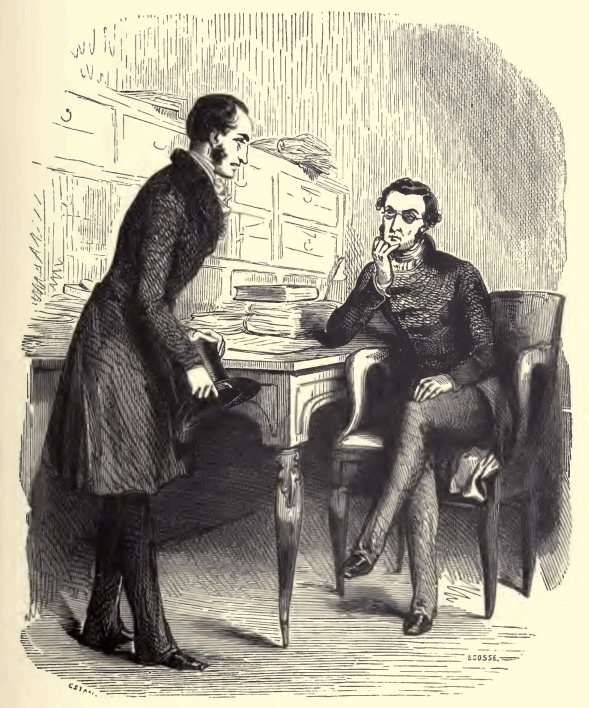
\includegraphics[width=\textwidth]{0161m.jpg}
\end{figure}

Villefort by a strong effort sought to control himself. “What is his
name?” said he. “Tell me his name.”

“Edmond Dantès.”

Villefort would probably have rather stood opposite the muzzle of a
pistol at five-and-twenty paces than have heard this name spoken; but
he did not blanch.

“Dantès,” repeated he, “Edmond Dantès.”

“Yes, monsieur.” Villefort opened a large register, then went to a
table, from the table turned to his registers, and then, turning to
Morrel,

“Are you quite sure you are not mistaken, monsieur?” said he, in the
most natural tone in the world.

Had Morrel been a more quick-sighted man, or better versed in these
matters, he would have been surprised at the king’s procureur answering
him on such a subject, instead of referring him to the governors of the
prison or the prefect of the department. But Morrel, disappointed in
his expectations of exciting fear, was conscious only of the other’s
condescension. Villefort had calculated rightly.

“No,” said Morrel; “I am not mistaken. I have known him for ten years,
the last four of which he was in my service. Do not you recollect, I
came about six weeks ago to plead for clemency, as I come today to
plead for justice. You received me very coldly. Oh, the royalists were
very severe with the Bonapartists in those days.”

“Monsieur,” returned Villefort, “I was then a royalist, because I
believed the Bourbons not only the heirs to the throne, but the chosen
of the nation. The miraculous return of Napoleon has conquered me, the
legitimate monarch is he who is loved by his people.”

“That’s right!” cried Morrel. “I like to hear you speak thus, and I
augur well for Edmond from it.”

“Wait a moment,” said Villefort, turning over the leaves of a register;
“I have it—a sailor, who was about to marry a young Catalan girl. I
recollect now; it was a very serious charge.”

“How so?”

“You know that when he left here he was taken to the Palais de
Justice.”

“Well?”

“I made my report to the authorities at Paris, and a week after he was
carried off.”

“Carried off!” said Morrel. “What can they have done with him?”

“Oh, he has been taken to Fenestrelles, to Pignerol, or to the
Sainte-Marguérite islands. Some fine morning he will return to take
command of your vessel.”

“Come when he will, it shall be kept for him. But how is it he is not
already returned? It seems to me the first care of government should be
to set at liberty those who have suffered for their adherence to it.”

“Do not be too hasty, M. Morrel,” replied Villefort. “The order of
imprisonment came from high authority, and the order for his liberation
must proceed from the same source; and, as Napoleon has scarcely been
reinstated a fortnight, the letters have not yet been forwarded.”

“But,” said Morrel, “is there no way of expediting all these
formalities—of releasing him from arrest?”

“There has been no arrest.”

“How?”

“It is sometimes essential to government to cause a man’s disappearance
without leaving any traces, so that no written forms or documents may
defeat their wishes.”

“It might be so under the Bourbons, but at present——”

“It has always been so, my dear Morrel, since the reign of Louis XIV.
The emperor is more strict in prison discipline than even Louis
himself, and the number of prisoners whose names are not on the
register is incalculable.” Had Morrel even any suspicions, so much
kindness would have dispelled them.

“Well, M. de Villefort, how would you advise me to act?” asked he.

“Petition the minister.”

“Oh, I know what that is; the minister receives two hundred petitions
every day, and does not read three.”

“That is true; but he will read a petition countersigned and presented
by me.”

“And will you undertake to deliver it?”

“With the greatest pleasure. Dantès was then guilty, and now he is
innocent, and it is as much my duty to free him as it was to condemn
him.” Villefort thus forestalled any danger of an inquiry, which,
however improbable it might be, if it did take place would leave him
defenceless.

“But how shall I address the minister?”

“Sit down there,” said Villefort, giving up his place to Morrel, “and
write what I dictate.”

“Will you be so good?”

“Certainly. But lose no time; we have lost too much already.”

“That is true. Only think what the poor fellow may even now be
suffering.”

Villefort shuddered at the suggestion; but he had gone too far to draw
back. Dantès must be crushed to gratify Villefort’s ambition.

Villefort dictated a petition, in which, from an excellent intention,
no doubt, Dantès’ patriotic services were exaggerated, and he was made
out one of the most active agents of Napoleon’s return. It was evident
that at the sight of this document the minister would instantly release
him. The petition finished, Villefort read it aloud.

“That will do,” said he; “leave the rest to me.”

“Will the petition go soon?”

“Today.”

“Countersigned by you?”

“The best thing I can do will be to certify the truth of the contents
of your petition.” And, sitting down, Villefort wrote the certificate
at the bottom.

“What more is to be done?”

“I will do whatever is necessary.” This assurance delighted Morrel, who
took leave of Villefort, and hastened to announce to old Dantès that he
would soon see his son.

As for Villefort, instead of sending to Paris, he carefully preserved
the petition that so fearfully compromised Dantès, in the hopes of an
event that seemed not unlikely,—that is, a second restoration. Dantès
remained a prisoner, and heard not the noise of the fall of Louis
XVIII.’s throne, or the still more tragic destruction of the empire.

Twice during the Hundred Days had Morrel renewed his demand, and twice
had Villefort soothed him with promises. At last there was Waterloo,
and Morrel came no more; he had done all that was in his power, and any
fresh attempt would only compromise himself uselessly.

Louis XVIII. remounted the throne; Villefort, to whom Marseilles had
become filled with remorseful memories, sought and obtained the
situation of king’s procureur at Toulouse, and a fortnight afterwards
he married Mademoiselle de Saint-Méran, whose father now stood higher
at court than ever.

And so Dantès, after the Hundred Days and after Waterloo, remained in
his dungeon, forgotten of earth and heaven.

Danglars comprehended the full extent of the wretched fate that
overwhelmed Dantès; and, when Napoleon returned to France, he, after
the manner of mediocre minds, termed the coincidence, \textit{a decree of
Providence}. But when Napoleon returned to Paris, Danglars’ heart
failed him, and he lived in constant fear of Dantès’ return on a
mission of vengeance. He therefore informed M. Morrel of his wish to
quit the sea, and obtained a recommendation from him to a Spanish
merchant, into whose service he entered at the end of March, that is,
ten or twelve days after Napoleon’s return. He then left for Madrid,
and was no more heard of.

Fernand understood nothing except that Dantès was absent. What had
become of him he cared not to inquire. Only, during the respite the
absence of his rival afforded him, he reflected, partly on the means of
deceiving Mercédès as to the cause of his absence, partly on plans of
emigration and abduction, as from time to time he sat sad and
motionless on the summit of Cape Pharo, at the spot from whence
Marseilles and the Catalans are visible, watching for the apparition of
a young and handsome man, who was for him also the messenger of
vengeance. Fernand’s mind was made up; he would shoot Dantès, and then
kill himself. But Fernand was mistaken; a man of his disposition never
kills himself, for he constantly hopes.

During this time the empire made its last conscription, and every man
in France capable of bearing arms rushed to obey the summons of the
emperor. Fernand departed with the rest, bearing with him the terrible
thought that while he was away, his rival would perhaps return and
marry Mercédès. Had Fernand really meant to kill himself, he would have
done so when he parted from Mercédès. His devotion, and the compassion
he showed for her misfortunes, produced the effect they always produce
on noble minds—Mercédès had always had a sincere regard for Fernand,
and this was now strengthened by gratitude.

“My brother,” said she, as she placed his knapsack on his shoulders,
“be careful of yourself, for if you are killed, I shall be alone in the
world.” These words carried a ray of hope into Fernand’s heart. Should
Dantès not return, Mercédès might one day be his.

\begin{figure}[ht]
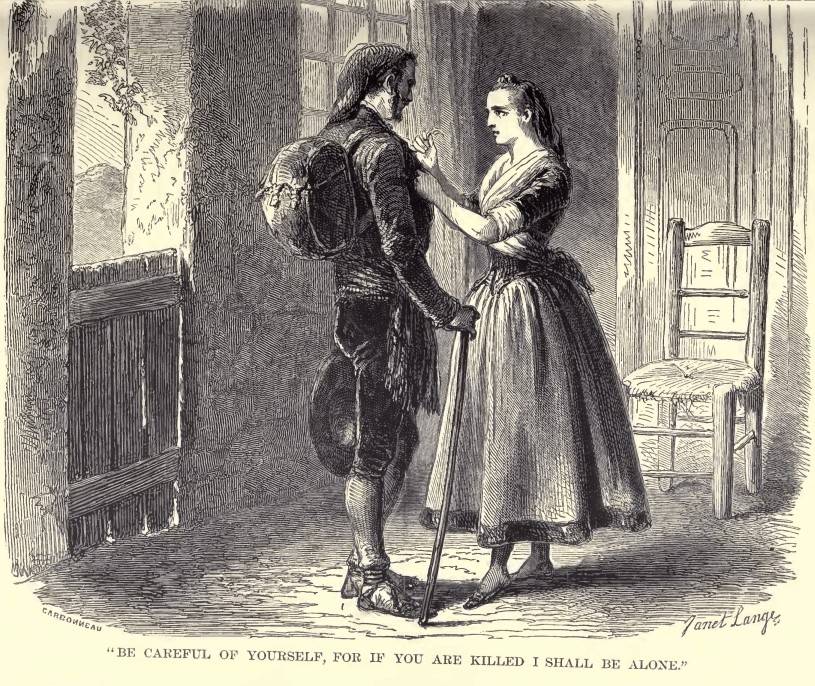
\includegraphics[width=\textwidth]{0165m.jpg}
\end{figure}

Mercédès was left alone face to face with the vast plain that had never
seemed so barren, and the sea that had never seemed so vast. Bathed in
tears she wandered about the Catalan village. Sometimes she stood mute
and motionless as a statue, looking towards Marseilles, at other times
gazing on the sea, and debating as to whether it were not better to
cast herself into the abyss of the ocean, and thus end her woes. It was
not want of courage that prevented her putting this resolution into
execution; but her religious feelings came to her aid and saved her.

Caderousse was, like Fernand, enrolled in the army, but, being married
and eight years older, he was merely sent to the frontier. Old Dantès,
who was only sustained by hope, lost all hope at Napoleon’s downfall.
Five months after he had been separated from his son, and almost at the
hour of his arrest, he breathed his last in Mercédès’ arms. M. Morrel
paid the expenses of his funeral, and a few small debts the poor old
man had contracted.

There was more than benevolence in this action; there was courage; the
south was aflame, and to assist, even on his death-bed, the father of
so dangerous a Bonapartist as Dantès, was stigmatized as a crime.
